\documentclass{article}

\usepackage{fullpage,verbatim,amsmath,graphicx,listings,color}

\newcommand{\HRule}{\rule{\linewidth}{0.5mm}}
\begin{document}

\lstset{
language=Python, 
basicstyle=\scriptsize,
backgroundcolor=\color{white},
showspaces=false,
showstringspaces=false,
showtabs=false,
frame=shadowbox,
tabsize=4,
captionpos=b,
title=\lstname,
breaklines=true,
breakatwhitespace=true}

\begin{titlepage}
 
\begin{center}
 
\textsc{\LARGE Homework 4}\\[1.5cm] 

\textsc{\Large Computational Math}\\[0.5cm]
 
 
\HRule \\[2cm]
 
% Author and supervisor
\begin{minipage}{0.4\textwidth}
\begin{flushleft} \large
\emph{Author:}\\
Mikola Lysenko
\end{flushleft}
\end{minipage}
 
\vfill
 
% Bottom of the page
{\large \today}
 
\end{center}
 
\end{titlepage}


\paragraph{1}

\subparagraph{a}
Let $u$ be a solution to the given ODE.  Then, for any $2\pi$ periodic smooth function $v$ it must be that:
\[ \int \limits_{-\pi}^{\pi} (u_{xx}(x) + \left( \sin(x) + \cos(x) + 2 \sin(x) \cos(x) \right) u(x)) v(x) dx = \int \limits_{-\pi}^{\pi} e^{\sin(x)} e^{\cos(x)} v(x) dx \]
By linearity, we can split the righthand side into homogeneous components and apply integration by parts.  For the second order components we get:
\begin{eqnarray*}
\int \limits_{-\pi}^{\pi} u_{xx}(x) v(x) dx & = & u_{x}(x)v(x) |_{-\pi}^{\pi} - \int \limits_{-\pi}^{\pi} u_{x}(x) v_x(x) dx \\
& = & -\int \limits_{-\pi}^{\pi} u_x(x) v_x(x) dx \\
& = & p_2(u, v)
\end{eqnarray*}

For the 0th order terms, no additional work is necessary to get a bilinear form:
\[ \int \limits_{-\pi}^{\pi} \left( \sin(x) + \cos(x) + 2 \sin(x) \cos(x) \right) u(x) v(x) dx = p_0(x) \]

And finally for the right hand side, we construct $f(v)$:
\[ \int \limits_{-\pi}^{\pi} e^{\sin(x)} e^{\cos(x)} v(x) dx = f(v) \]

By construction our space of test functions satisifies the boundary, so we have the following weak form for the system:
\[ u^T (p_2 + p_0) v = f^T v \]

\subparagraph{b}

Fix a collection of $n$ ordered grid points $X = \{ x_i \in [-\pi, \pi) | x_i < x_{i+1}, i \in [0,N) \}$.  To get a cG(1) finite element discretization, we restrict the space of test functions and solutions to piecewise linear maps over this grid, which is spanned by the basis of hat functions.  We define the $i^{th}$ basis hat function, $\varphi^i(x)$, as follows:

\[ \varphi^i(x) = \left \{ \begin{array}{cc}
\frac{x_{i+1} - x}{x_{i+1} - x_{i}} & \textrm{if } x \in [x_{i},   x_{i+1}) \\
\frac{x - x_{i-1}}{x_{i} - x_{i-1}} & \textrm{if } x \in [x_{i-1}, x_{i})   \\
0 & \textrm{otherwise}
\end{array} \right. \]

Boundary conditions are applied to make the test functions cyclic.  This may be done by just taking the indexes mod $n$ and the difference terms mod $2 \pi$.  Substituting this into the above equation gives the following matrix equation for the discrete Galerkin equation:

\[ p_2(\varphi^i, \varphi^j) + p_0(\varphi^i, \varphi^j) = f(\varphi^j) \]

Now we expand each term separately and integrate piecewise.  Starting with $p_2$:

\begin{eqnarray*}
p_2(\varphi^i, \varphi^j) & = & - \int \limits_{-\pi}^{\pi} \varphi^i_x(x) \varphi^j_x(x) dx \\
& = & \left( \delta_{i,j+1} - \delta_{i,j} \right) \int \limits_{x_{i-1}}^{x_{i}} \left( \frac{1}{x_{i} - x_{i-1}} \right)^2 dx 
+ \left( \delta_{i,j-1} - \delta_{i,j} \right) \int \limits_{x_{i}}^{x_{i+1}}  \left( \frac{1}{x_{i+1} - x_{i}} \right)^2 dx \\
& = & \left( \delta_{i,j+1} - \delta_{i,j} \right) \frac{1}{x_{i} - x_{i-1}} 
+ \left( \delta_{i,j-1} - \delta_{i,j} \right) \frac{1}{x_{i+1} - x_{i}}
\end{eqnarray*}

Next we deal with $p_0$:
\begin{eqnarray*}
p_0(\varphi^i, \varphi^j) & = & \int \limits_{-\pi}^{\pi} \left( \sin(x) + \cos(x) + 2 \sin(x) \cos(x) \right) \varphi^i(x) \varphi^j(x) dx\\
 & = & 
\int \limits_{x_{i-1}}^{x_i} \left( \sin(x) + \cos(x) + 2 \sin(x) \cos(x) \right) \frac{ (x - x_{i-1}) (\delta_{i,j} (x - x_{i-1}) + \delta_{i,j+1}(x_i - x)) }{\left(x_{i} - x_{i-1}\right)^2} dx + \\
& & \int \limits_{x_{i}}^{x_{i+1}} \left( \sin(x) + \cos(x) + 2 \sin(x) \cos(x) \right) \frac{ (x_{i+1} - x) (\delta_{i,j} (x_{i+1} - x) + \delta_{i,j-1}(x - x_i))}{\left(x_{i} - x_{i+1}\right)^2} dx
\end{eqnarray*}

And finally $f$:
\begin{eqnarray*}
f(\varphi^i) & = & \int \limits_{-\pi}^{\pi} e^{\sin(x) + \cos(x)} \varphi^i(x) dx \\
& = & \int \limits_{x_{i-1}}^{x_i} e^{\sin(x) + \cos(x)} \frac{x - x_{i-1}}{x_{i} - x_{i-1}} dx + \int \limits_{x_{i}}^{x_{i+1}} e^{\sin(x) + \cos(x)} \frac{x_{i+1} - x}{x_{i+1} - x_{i}} dx
\end{eqnarray*}

Putting this together, we get the following coefficient matrix, $M_{i,j}$, such that:
\begin{eqnarray*}
M_{i,j} & = & p_2(\varphi^i, \varphi^j) + p_0(\varphi^i, \varphi^j)
\end{eqnarray*}

And for the right hand side, we get $b_i$ such that:
\begin{eqnarray*}
b_i & = & f(\varphi^i)
\end{eqnarray*}

And so the final problem is to solve for some coefficients $u^i$ such that:
\[ M u = b \]

\subparagraph{c}

To evaluate the integrals in part b, we use numerical quadrature (except for the Laplacian term, which is trivial).  Here is my code (written in python using SciPy, PyLab and Sympy):

\pagebreak
\lstinputlisting{prob1.py}

And here is the output plot of the computed solution compared to the exact solution, $u(x) = \exp( \sin(x) + \cos(x) )$:

\begin{center}
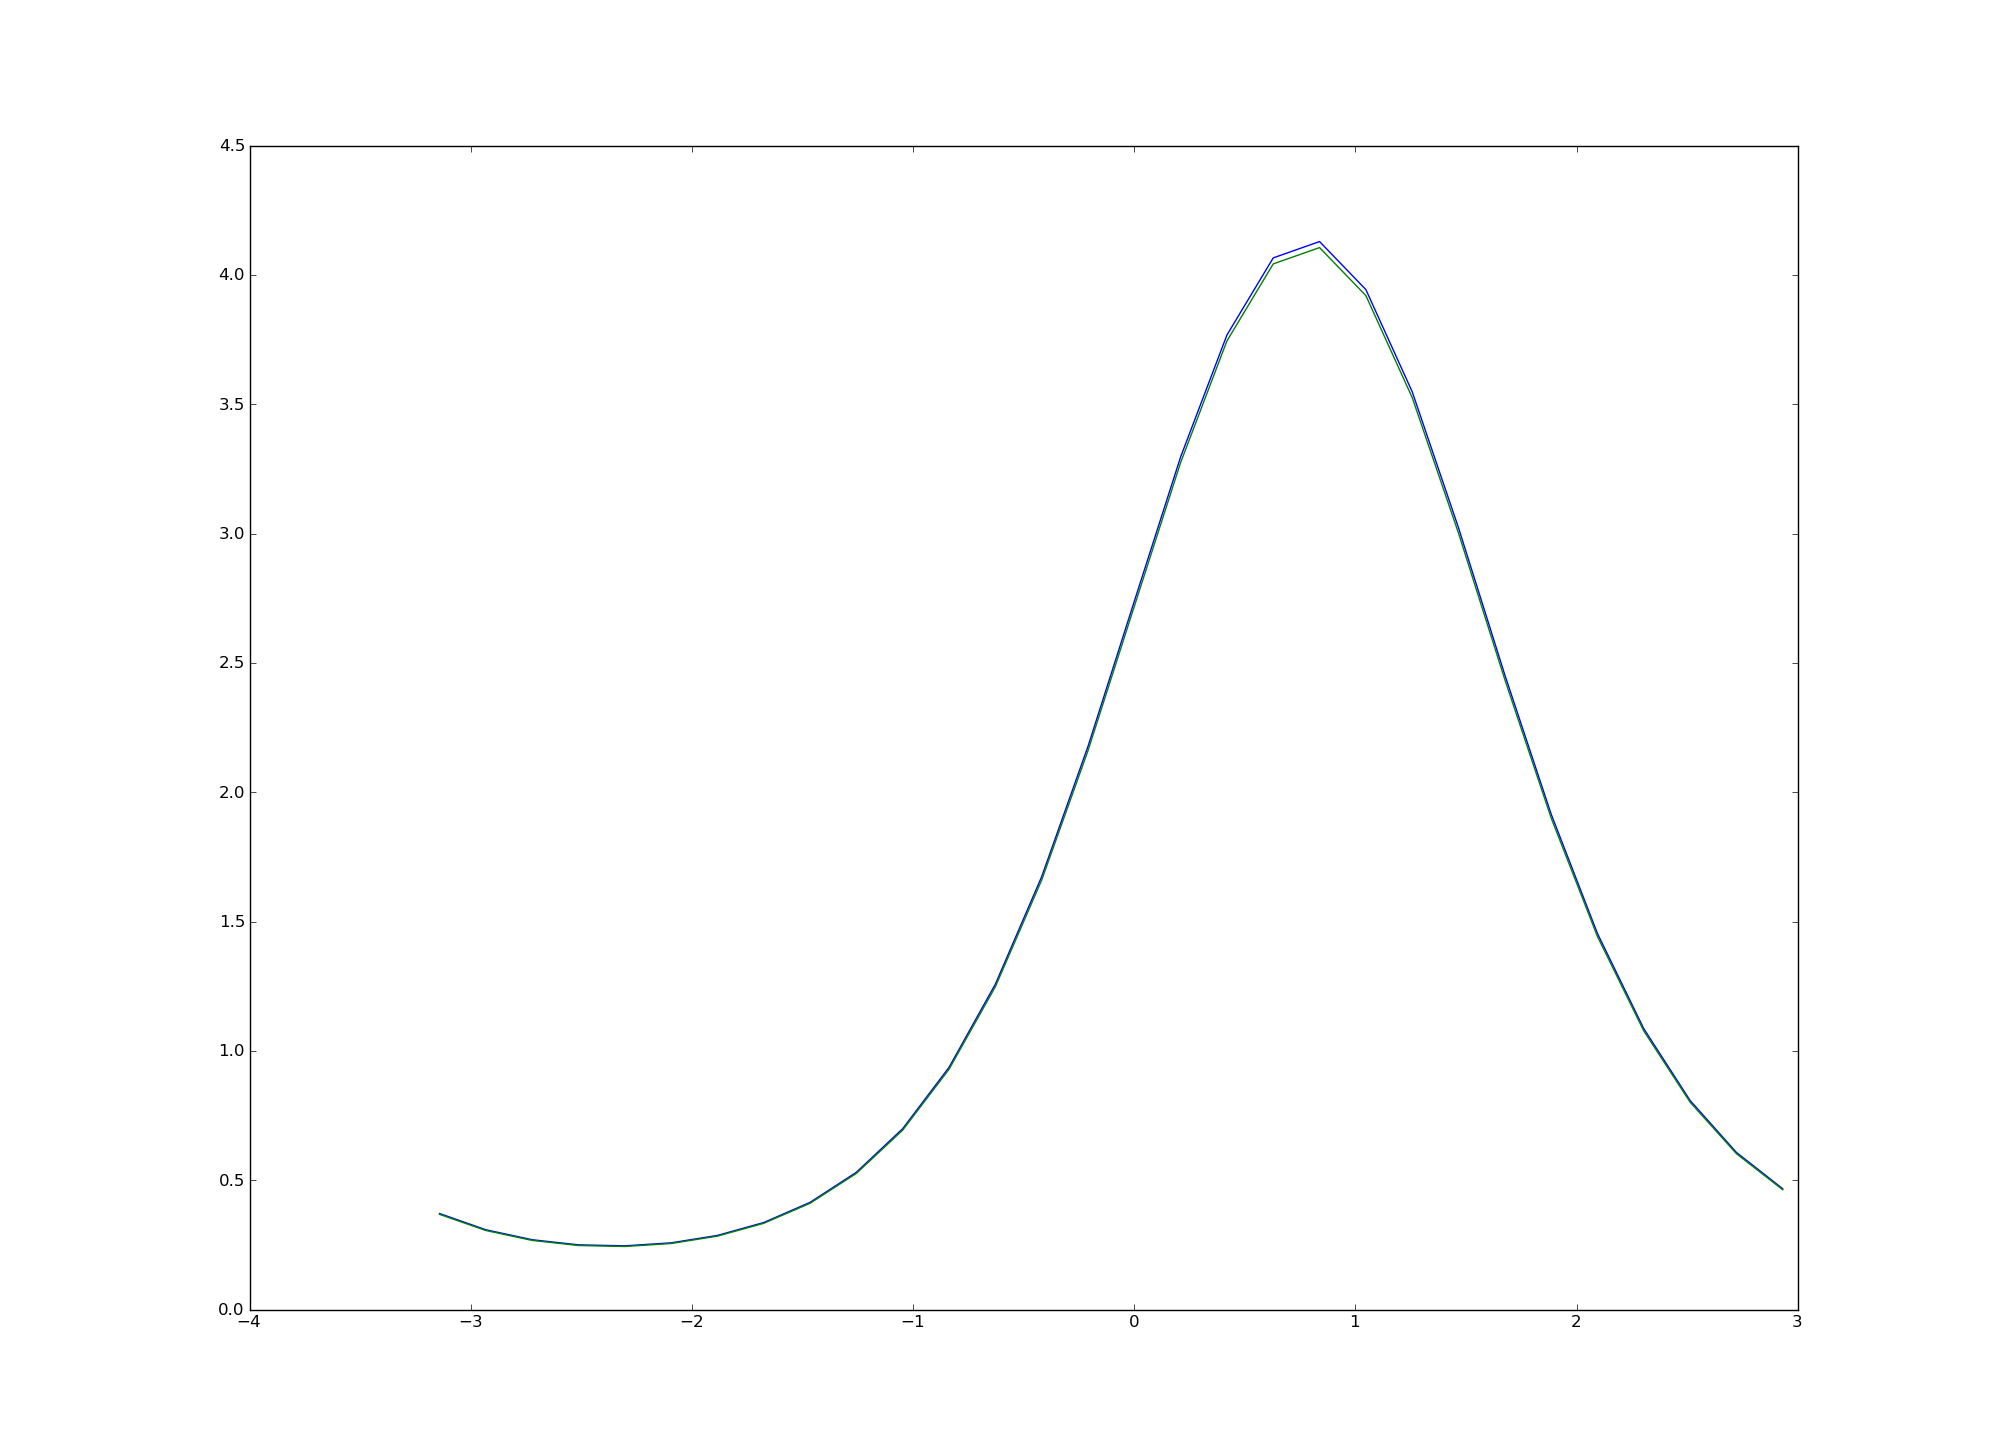
\includegraphics[width=4in]{prob1_result.png}
\end{center}

\paragraph{2}

\subparagraph{a}

To start with, we modify $p_0$ and $f$ from part 1, giving the following new form for $M$ and $b$:
\[ M_{i,j} = \]

And:
\[ b_i = \]

To compute the error within the $i^{th}$ node we do 'blah'

\subparagraph{b}

\subparagraph{c}

\end{document}
